\section{Design and Implementation}
\label{sec:implementation}
In the following I will present a bunch of noteworthy implementation details.

\subsection{Extraction Templates}
As mentioned in Section~\ref{sec:wiktionary}, we define \textit{block} as the part of the hierarchical page that is responsible for a certain entity in the extracted RDF graph. 
For each \textit{block}, there can be declarations on how to process the page on that level.
This is done by so called \textit{extraction templates}(ET) (not to be confused with the templates of \textit{wikitext} .
Each possible section in the \wik page layout (i.e. each linguistic property) has an ET configured (explained in detail below). 
The idea is to provide a declarative and intuitive way to encode \textit{what to extract}.
For example consider the following page snippet:
\begin{lstlisting}
===Synonyms===
* [[building]]
* [[company]]
\end{lstlisting}
Since the goal is to emit a link to each resource per line, we can write the ET in the following style (using the popular scraping paradigms such as regular expressions):
\begin{lstlisting}
===Synonyms===
(* [[\$target]]
)+
\end{lstlisting}
Some simple constructs for variables ( ``\texttt{\$target}'') and loops (``\texttt{(*}'', ``\texttt{)+}'') are defined for the ET syntax.
If they are \textit{matched against} an actual wiki page, \textit{bindings} are extracted by a matching algorithm.
We omit a low-level, technical description of the algorithm --- one can think of it like a Regular Expression \textit{Named Capturing Group}.
The found \textit{variable bindings} for the above example are \texttt{\{(target->building), (target->company)\}}. 
The triple generation rule encoded in XML looks like:
\begin{lstlisting}[style=XML]
<triple s="http://some.ns/$entityId" p="http://some.ns/hasSynonym" o="http://some.ns/$target" />
\end{lstlisting}
Notice the reuse of the \texttt{\$target} variable:
The data extracted from the page is inserted into a triple.
The variable \texttt{\$entityId} is a reserved global variable, that holds the page name e.g. the word.
The created triples in N-Triples syntax are:
\begin{lstlisting}[style=N3]
<http://some.ns/house-1>   <http://some.ns/hasSynonym>   <http://some.ns/building> .
<http://some.ns/house-1>   <http://some.ns/hasSynonym>   <http://some.ns/company> .
\end{lstlisting}
The actual patterns are more complex (as explained below), but the mechanism is consistently used throughout the system.

\subsection{Algorithm}
The algorithm of processing a page works as follows:

\textit{Input:} Parsed page obtained from the DBpedia Framework (essentially a lexer is used to split the Wiki Syntax into tokens)
\begin{enumerate}
\item Filter irrelevant pages (user/admin pages, statistics, list of things, files, templates, etc.) by applying string comparisons on the page title. Return an empty result on that condition.
\item Build a finite state automaton\footnote{Actually a finite state transducer, most similar to the Mealy-Model.} from the page layout encoded in the WLE specific XML configuration. This schema also contains so called \textit{indicator templates} for each \textit{block}, that --- if they match at the current page token --- indicate that their respective block starts. 
So they trigger state transitions. In this respect the mechanism is similar to \cite{McCrae_2012}, but in contrast our approach is declarative --- the automaton is constructed \textit{on-the-fly} and not hard-coded. 
The current state represents the current position in the disambiguation tree.
\item The page is processed token by token:
\begin{enumerate}
\item Check if \textit{indicator templates} match. 
If yes, the corresponding block is entered. 
The \textit{indicator templates} also emit triples like in the \textit{extraction template} step below. 
These triples represent the block in RDF -- for example the resource \url{http://wiktionary.dbpedia.org/resource/semantic-English} represents the English block of the page "semantic".
\item Check if any \textit{extraction template} of the current block match.
\subitem If yes, transform the variable bindings to triples.\footnote{In our implementation: 
Either declarative rules are given in the XML config or alternatively static methods are invoked on user-defined classes (implementing a special interface) for an imperative transformation. This can greatly simplify the writing of complex transformation.} Localization specific tokens are replaced as configured in the so called \textit{language mapping} (explained in detail in section \ref{sec:mapping}).
\end{enumerate}
\item The triples are then \textit{transformed}. In our implementation \textit{transformation} means, that all triples are handed to a static function, which return a set of triples again. One could easily load the triples into a triple store like JENA and apply arbitrary SPARQL Construct and Update transformations. 
This step basically allows post-processing, e.g. consolidation, enrichment or annotation. 
In our case, we apply the schema transformation (by the mediator) explained in detail in Section \ref{sec:lemon}).
\item The triples are sorted and de-duplicated to remove redundancy in the RDF dumps.
\end{enumerate}
\textit{Output:} Set of triples (handed back to the DBpedia Framework).

\subsection{Language Mapping}\label{sec:mapping}
The language mappings are a very simple way to translate and normalize tokens, that appear in a WLE. 
In the German WLE, for example, a noun is described with the German word "\textit{Substantiv}". 
Those tokens are translated to a shared vocabulary, before emitting them (as URIs for example). 
The configuration is also done within the language specific XML configuration:
\begin{lstlisting}[style=XML]
 <mapping from="Substantiv" to="Noun"> 
 <mapping from="Deutsch" to="German"> 
 ...
\end{lstlisting}
The mapping consists currently of mappings for part of speech types and languages. But arbitrary usage is possible. Section~\ref{sec:functions} shows how this mapping is used.

\subsection{Reference Matching}\label{sec:matching}
A \wik specific requirement is the resolution of intra-page references: All Wiktionaries use \textit{some} way to refer to parts of the traits of the word. For example on the page \textit{house} at first senses are defined:
\begin{lstlisting}[basicstyle=\tiny\ttfamily]
# A structure serving as an [[abode]] of human beings.
# {{politics}} A deliberative assembly forming a component of a legislature, or, more rarely, the room or building in which such an assembly normally meets.
# [[house music|House music]].
\end{lstlisting}
Later on relations to other words are noted --- but \textit{in context} of a sense. For example house \textit{in context} of \textit{abode} has the translation \textit{Haus} in German. So the following notion is used:
\begin{lstlisting}[basicstyle=\tiny\ttfamily]
====Translations====
{{trans-top|abode}}
...
* German: {{t+|de|Haus|n}}, {{t+|de|Häuser|p}}
...
\end{lstlisting}
The problem is to match the gloss that is given in the \texttt{trans-top} template argument against the available senses. There is no simple way to determine that. As described in \cite{meyer_2011b} as \textit{relation anchoring}, a string based measure is used\footnote{Opposed to the approach described in \cite{meyer_2011b}, we only rely on information actually encoded on the page, the source of the link is determined by the position in the disambiguation tree and sense definitions. But a \textit{target anchoring} --- is not performed. \textit{Target anchoring} refers to the disambiguation of the target word (or entity): this target of course has also a disambiguation tree, and it is possible to \textit{bend} the link to point to a node deeper in that tree instead of just the root node. We consider this highly assumptious and it introduces noise. We leave that to postprocessing. Also it is not implementable easily within the DBpedia framework, because data extracted on other pages is not available to a extractor at runtime.}. There is a simple data structure that is initialized per page, to this matching mechanism. Which measure is used can be configured in the global configuration. Available measures are: Levenshtein and trigram set similarity with dice, jaccard or overlap coefficient. A sense can be registered with the matcher by passing its definition sentence. An \textit{id} is generated for that sense. Later on, glosses (short forms of the definition) that refer to a sense can be passed to lookup which sense matches best, and the corresponding \textit{id} is returned. Section~\ref{sec:functions} shows how this mechanism is used.


\subsection{Formatting functions in Result Templates}\label{sec:functions}
The question arises, how this mapping is then used within the application. It is certainly not reasonable to replace \textit{all} occurrences of those \texttt{from} tokens. This would lead to a number of false positive matches and screwed output. It is crucial to offer a possibility to configure in which context output should be handled so.
I therefore introduced formatting functions in result templates: when you note the triples that are generated you can apply functions to e.g. variables. An example:
\begin{lstlisting}[style=XML]
<triple s="http://some.ns/uri($entityId)" p="http://some.ns/hasLanguage" o="http://some.ns/map($target)" />
\end{lstlisting}
In this RT, two functions are used: \texttt{uri} and \texttt{map}. They are wrapped around variable parts, and on rendering they are resolved. The following functions are available:\\
\begin{table}[h!] 
\centering 
\begin{tabular}{|l|l|}
\hline \texttt{uri(str)} & URL encode \\ 
\hline \texttt{map(str)} & replace if mapping found \\ 
\hline \texttt{assertMapped(str)} & dont emit triple if not in mapping vocabulary \\ 
\hline \texttt{assertNumeric(str)} & dont emit triple if argument is not numeric \\ 
\hline \texttt{getId(str)} & lookup a gloss and return the id of the best matching sense \\ 
\hline \texttt{getOrMakeId(str)} & lookup a id or generate one if below a similarity threshold \\ 
\hline \texttt{makeId(str)} & save a sense and generate an id \\ 
\hline \texttt{saveId(str, str)} & save a sense with a given id \\ 
\hline 
\end{tabular} 
\end{table}
The functions with \textit{Id} in their name relate to the matching introduced in section~\ref{sec:matching}. Continuing the example of senses and translations, one would write the RT in a way to save definition sentences when generating them as triples and later matching the gloss, when generating triples about the translation section:
For the defintions
\begin{lstlisting}[style=XML]
<triple s="http://some.ns/$entityId-makeId($definition)" p="http://some.ns/hasDefinition" o="$definition" oType="literal" />
\end{lstlisting}
and for the translations
\begin{lstlisting}[style=XML]
<triple s="http://some.ns/$entityId-getId($gloss)" p="http://some.ns/hasTranslation" o="http://some.ns/uri($target)" />
\end{lstlisting}
The idea is that (if the matching is correct), the subject URIs are equal (e.g. \url{http://some.ns/house-1}) in both triples --- there are two triples about one resource --- information successfully merged.
\begin{lstlisting}[style=N3]
<http://some.ns/house-1>   <http://some.ns/hasDefinition>   "A structure serving as an abode of human beings." .
<http://some.ns/house-1>   <http://some.ns/hasTranslation>   <http://some.ns/Haus> .
\end{lstlisting}
 
\subsection{Schema Mediation by Annotation with \lemonnospace}
\label{sec:lemon}
The last step of the data integration process is the schema normalization.
The global schema of all WLE is not constructed in a centralized fashion --- instead we found a way to both making the data globally navigable and keeping the heterogeneous schema without loosing information.
\lemonnospace~\cite{lemon-eswc} is an RDF model for representing lexical information (with links to ontologies --- possibly DBpedia). 
We use part of that model to encode the relation between \textit{lexical entries} and \textit{lexical senses}.
\lemon has great potential of becoming the \textit{de facto} standard for representing dictionaries and lexica in RDF and is currently the topic of the OntoLex W3C Community group\footnote{\url{http://www.w3.org/community/ontolex/}}. 
The rationale is to add \textit{shortcuts} from \textit{lexical entities} to \textit{senses} and propagate properties that are along the intermediate nodes down to the senses.
This can be accomplished with a generic algorithm (a generic tree transformation, regardless of the depth of the tree and used links).
Applications assuming only a \textit{lemon} model, can operate on the shortcuts and (if applied as an overlay --- leaving the original tree intact) this still allows applications, to also operate on the actual tree layout.
The (simplified) procedure is presented in Figure~\ref{fig:lemon}\footnote{Note, that in the illustration it could seem like the information about part-of-speech would be missing in the \textit{lemon} model. This in not the case. Actually from the part-of-speech nodes, there is a link to corresponding language nodes.
These links are also propagated down the tree.}. 
\begin{figure}[tb]
\centering
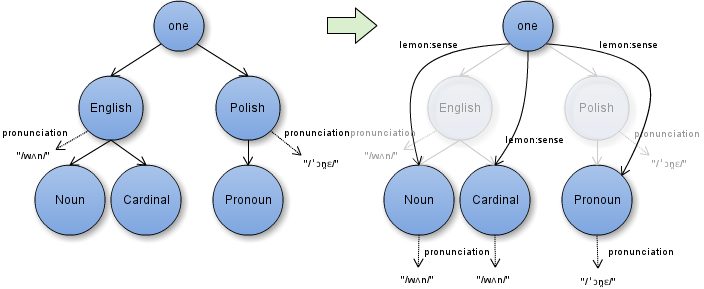
\includegraphics[width=\textwidth]{./images/lemon.png}
\caption{Schema normalization.}
\label{fig:lemon}
\end{figure}
The use of the \lemon vocabulary and model as an additional schema layer can be seen as our mediator.
This approach is both lightweight and effective as it takes advantage of \textit{multi-schema modelling}.

\subsection{Configuration}
As presented in section \ref{sec:requirements}, the most important requirement of the approach is configurability. The extractor itself is as generic as possible, it is not tailored to linguistics or even \wik. It has commitment to wiki syntax, but is also able to process plain text as it can be interpreted as wikitext without markup, thus the extractor may be suitable for most flat file formats. However the configuration makes up the heart of the extractor: it is a big XML file interpreted at runtime and describes how to interpret the page. I will go through the available options and show their relevance to the given requirements.

At first the configuration is splitted into a generic part and a language specific part. The generic part is always loaded and does not need to be localized to a WLE. It contains options like the namespace, in which all URIs are created and an option that specifies which language configuration should be used. The language specific configuration is loaded based on that option at runtime. It has to be tailored to a WLE by the maintainer of the dataset.

Both configuration types are stored in the \texttt{config} folder. The naming convention restricts the folder to like the following:
\dirtree{%
.1 config.
.2 config.xml.
.2 config-de.xml.
.2 config-en.xml.
.2 \ldots.
}

The generic configuration has two parts: a properties list and a mapping. The properties are the mentioned namespace, the language, the \texttt{loglevel} (to configure debug verbosity) and options to configure the matcher. The mapping is --- as explained in section~\ref{sec:mapping} --- a way to replace tokens found on the page to a global vocabulary. But opposed to language specific tokens, in the generic configuration, globally used tokens are configured. It is used to provide a mapping from ISO 639-1 and -2 codes to the \wik vocabulary.

\begin{lstlisting}[style=XML]
<?xml version="1.0" encoding="UTF-8"?>
<config>
    <properties>
        <property name="logLevel" value="0"/>
        <property name="language" value="ru"/>
        <property name="ns" value="http://wiktionary.dbpedia.org/"/>
        <property name="matchingStrategy" value="levenshtein"/>
        <property name="matchingThreshold" value="0.5"/>
    </properties>
    <mappings>
        <!-- ISO 639-1 -->
        <mapping from="aa" to="Afar" />
        <mapping from="ab" to="Abkhazian" />
        <mapping from="ae" to="Avestan" />
        ...
\end{lstlisting}



\newpage

